\documentclass{SelimArticle}
%!TEX root = main.tex

%%%%%%%%%%%%%%%%%%%%%%%%%%%%%%%
% Additional Packages/Options %
%%%%%%%%%%%%%%%%%%%%%%%%%%%%%%%
% \setlist{nosep}
\hypersetup{hidelinks}

%%%%%%%%%%%%%%%%%
% Title Options %
%%%%%%%%%%%%%%%%%
\usepackage{mypage}
\school{McGill University}
\course{Computational Aerodynamics}
\coursenum{MECH 539}
%Add \\[0.3cm] for new line.
\title{Project 5}
\student{Selim \textsc{Belhaouane}}
\studentnum{260450544}
\date{\today}

%%%%%%%%%%%%%%%%%%%%%%%%%
% Additional Formatting %
%%%%%%%%%%%%%%%%%%%%%%%%%
%Horizontal line below section.
\sectionfont{\sectionrule{0pt}{0pt}{-5pt}{0.8pt}}
%Section numbering depth. Value of 2 means numbering ends with subsections.
\setcounter{secnumdepth}{3}
%Table of contents section depth. Same as above.
\setcounter{tocdepth}{2}
\numberwithin{equation}{section}
\numberwithin{figure}{section}

\newcommand{\ra}[1]{\renewcommand{\arraystretch}{#1}}
\newcommand{\pdiff}[2]{\ensuremath{
    \frac{\partial #1}{\partial #2}
}}
\newcommand{\ip}{\ensuremath{_{i+1,j}}}
\newcommand{\im}{\ensuremath{_{i-1,j}}}
\newcommand{\jp}{\ensuremath{_{i,j+1}}}
\newcommand{\jm}{\ensuremath{_{i,j-1}}}
\begin{document}
\mytitlepage
% \tableofcontents
\newpage
% Begin writing here.
\section{Nomenclature}
$N$ is the number of grid points in one direction, i.e. a 400x400 grid corresponds to
$N = 400$.
\section{Governing Differential Equation}
The Laplace equation in two dimensions is given by:
\begin{equation}
    \label{eq:laplace}
    \frac{\partial^2 u}{\partial x^2} + \frac{\partial^2 u}{\partial y^2} = 0
\end{equation}
The boundary conditions are:
\begin{gather*}
    u(x,0) = u(0,y) = u(1,y) = 0\\
    u(x,1) = 1
\end{gather*}

\section{Question 1}
\begin{quote}
    \textit{
     Derive the truncation error for the second-order finite-difference spatial discretization
     for the Laplace equation.}
\end{quote}
A second-order finite-difference spatial discretization for a second derivative is given by:
\begin{equation}
    \label{eq:secord}
    \pdiff{^2u}{x^2} = \frac{u\ip^n - 2 u_{ij}^n + u\im^n}{\Delta x^2}
\end{equation}
Thus, plugging~\Cref{eq:secord} into~\Cref{eq:laplace} yields the following discretization:
\begin{equation}
    \label{eq:laplacediscrete}
    \frac{u\ip^n - 2 u_{ij}^n + u\im^n}{\Delta x^2}
    + \frac{u\jp^n - 2 u_{ij}^n + u\jm^n}{\Delta y^2} = 0
\end{equation}
Now, we substitute each term by its Taylor series expansion into~\Cref{eq:laplacediscrete} to obtain
the modified equation:
\begin{equation*}
    \label{eq:te}
    u_{xx} + u_{yy} =
    \underbrace{
        - \frac{1}{12}\left(u_{xxxx}\Delta x ^2 + u_{yyyy}\Delta y^2 \right)
        + O(\Delta x^4, \Delta y^4)
    }_{\text{Truncation Error}}
\end{equation*}
Note the leading error terms are a function of $\Delta x^2, \Delta y^2$, hence the scheme being
second-order accurate.
\section{Question 2}
\begin{quote}
    \textit{Derive the modified equation for the scheme and note whether the error is dissipative,
    dispersize, or a combination of the two. Explain why?}
\end{quote}
As derived in the previous question, the truncation error is given by:
$$
    \frac{1}{12}\left(u_{xxxx}\Delta x ^2 + u_{yyyy}\Delta y^2 \right)
    + O(\Delta x^4, \Delta y^4)
$$
Due to the discretization, all the odd-order derivatives vanish, leaving only the even-order ones.
Now, we know that a second-order derivative in the truncation error introduces dissipation.
The same can be said of all even-order derivatives.

Thus, the chosen scheme induces dissipative errors \textbf{only}.

\section{Solver Parameters}
Before moving on to the numerical questions, it is important to state all solver parameters.
\begin{description}[noitemsep]
    \item[Programming Language:] Fortran90
    \item[Compiler:] GNU Fortran
    \item[Optimization Level:] O3 (fastest), unless otherwise specified
    \item[Precision:] Double
    \item[Convergence Criteria:] $r^{(k+1)} < 10^{-6}$
    \item[Relaxation Parameter:] 1.5, unless otherwise specified
\end{description}

The residual for each iteration is calculated as:
$$
r^{(k+1)} = \max_{ij}\left( u^{(k+1)}_{ij} - u^{(k)}_{ij} \right)
$$
\newpage
\section{Question 3}
\begin{quote}
    \textit{Demonstrate the solution of the Laplace Equation for the 400}x\textit{400.}
\end{quote}
The solution of the Laplace Equation is given in~\Cref{fig:q3}.
\begin{figure}[H]
    \centering
    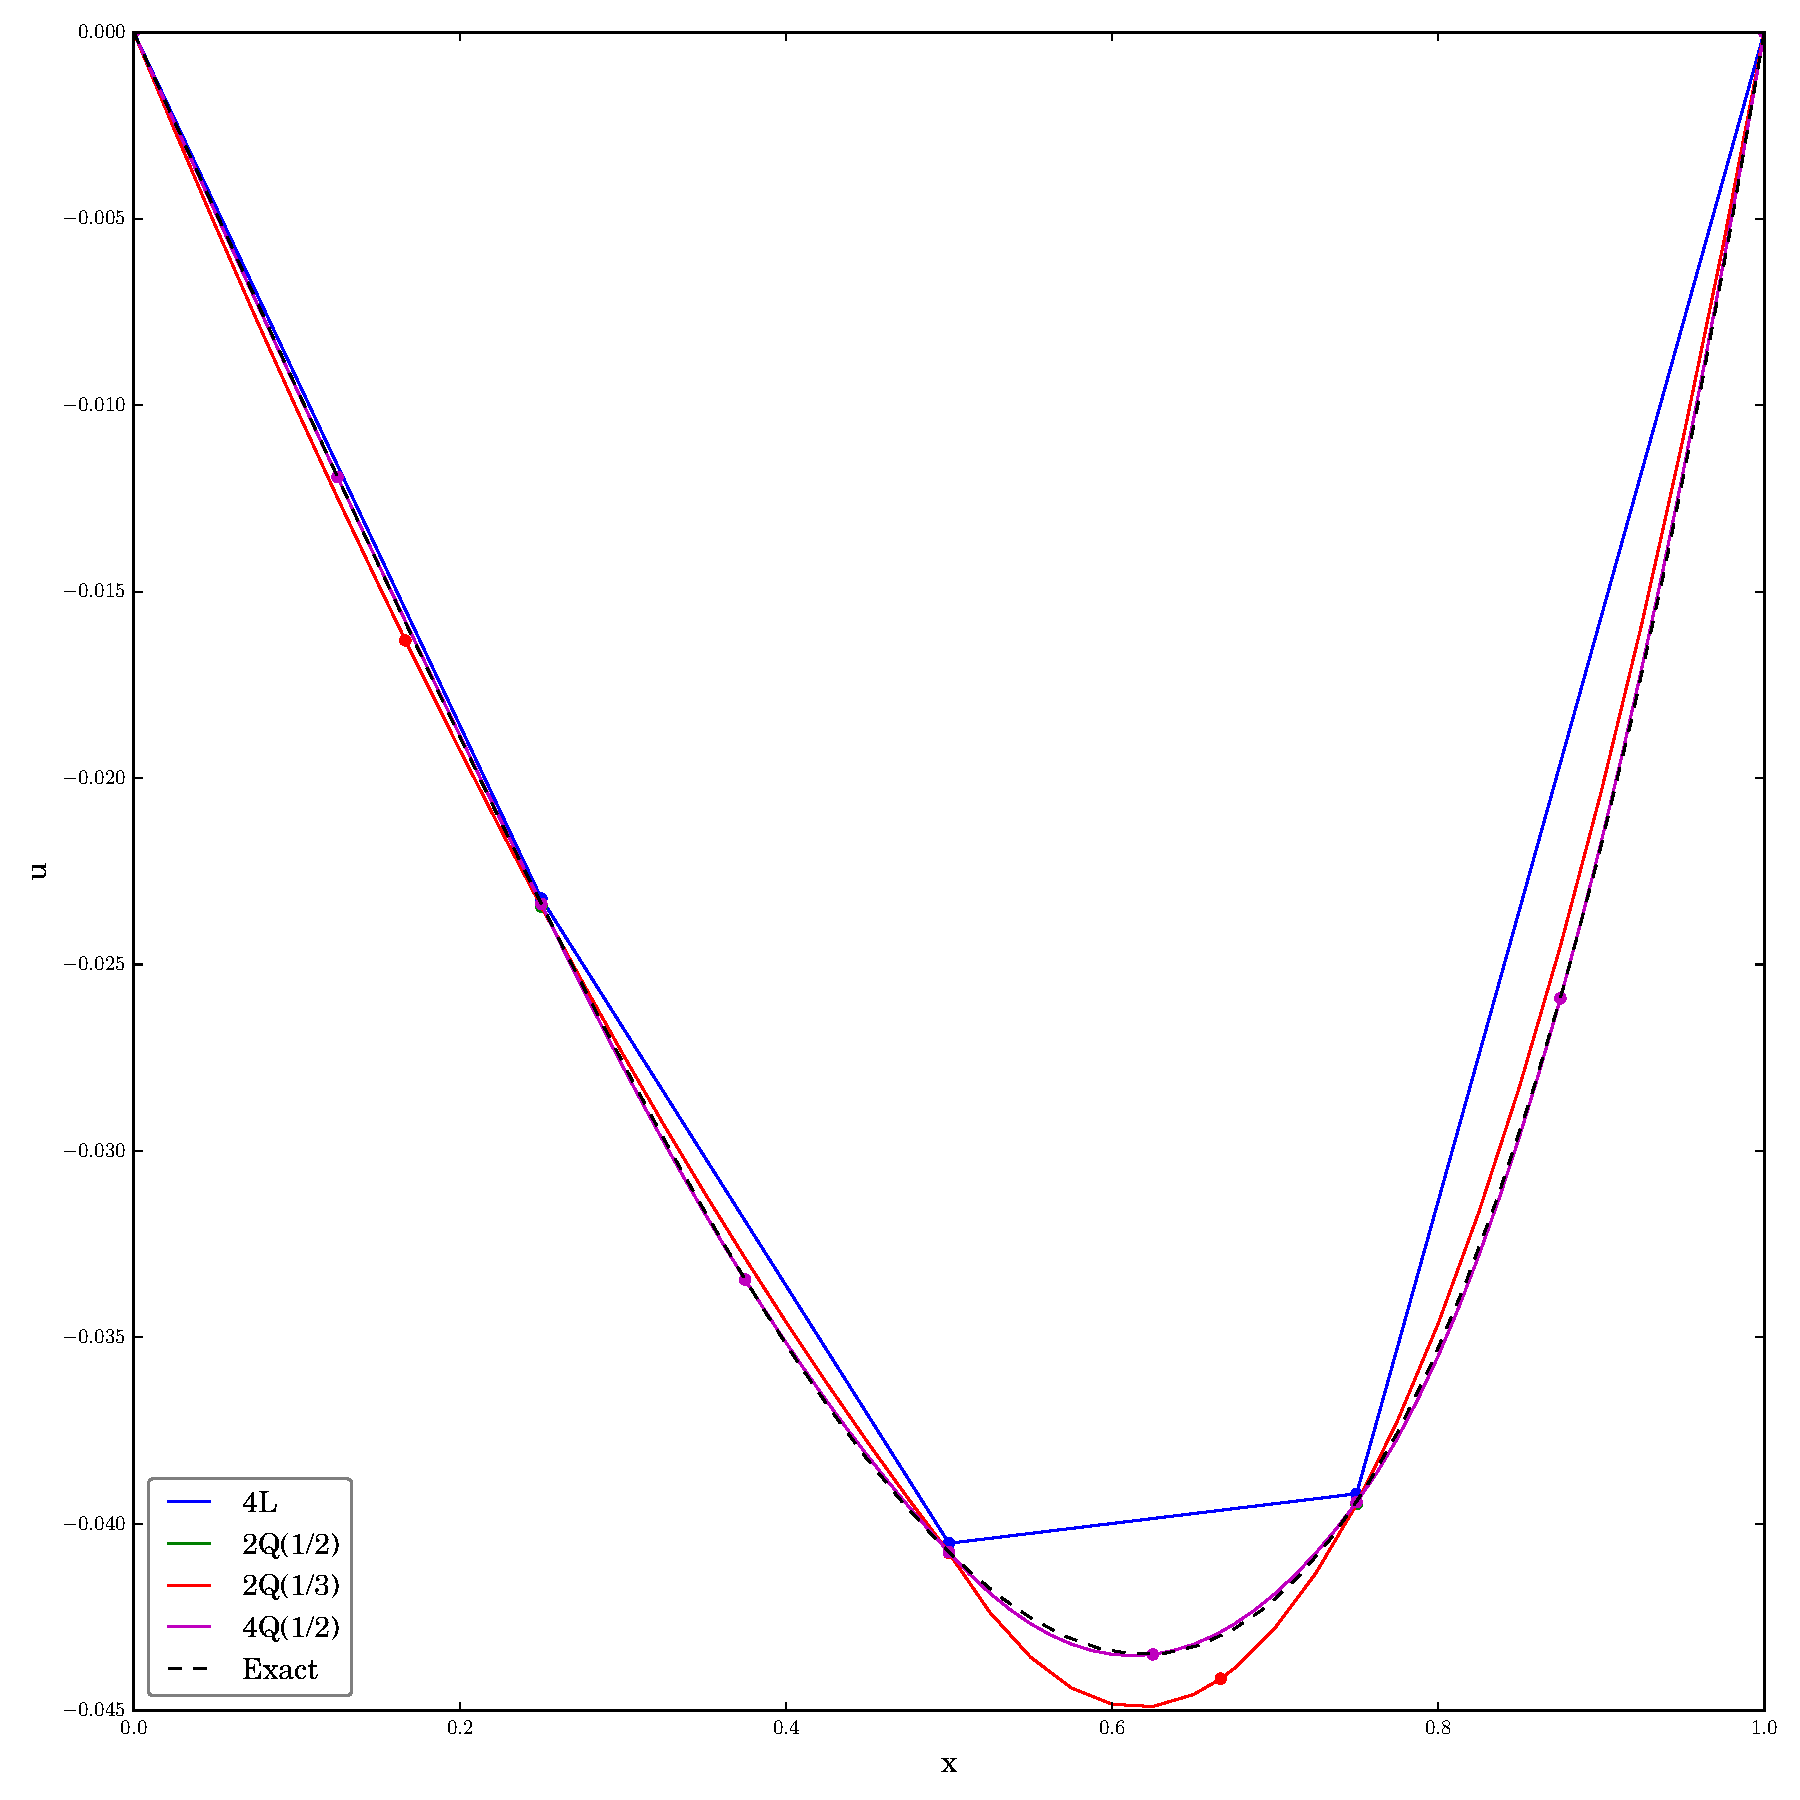
\includegraphics[width=0.8\textwidth]{./figs/q3.pdf}
    \caption{Solution of the Laplace Equation}\label{fig:q3}
\end{figure}

\newpage
\section{Question 4}
\begin{quote}
\textit{
    Convergence of the residual versus the number of iterations for all three
    methods on the same plot. Provide a plot for each grid size. Discuss the
    difference between the schemes.  Compute the condition number of the
    matrix using the Forsythe-Moler method and discuss the results.
}
\end{quote}
Refer to~\Cref{fig:q4} for the convergence plots.

\begin{figure}
    \centering
    \includegraphics[width=1.0\textwidth]{./figs/q4.pdf}
    \caption{Convergence history comparison between methods for $N = 100, 200, 400$  going from top to bottom.}\label{fig:q4}
\end{figure}
\subsection{Effect of scheme on convergence}
It can be seen that the Jacobi scheme is consistently slower to converge than the other schemes, whereas
SOR is the fastest. However the chosen relaxation parameter plays a significant role in the convergence rate
for the latter scheme, as will be shown for Question 7.

It is not a surprise that the Gauss-Siedel scheme is faster than Jacobi due to the former using
more up-to-date information, i.e. $u^{(k+1)}$ values, which leads to a greater rate of ``information spreading'' over
the problem domain.

Again, the reason for SOR's even faster convergence rate is given in Question 7.

\subsection{Effect of grid size on convergence}
From a purely physical point of view, one would expect the number of iterations required to converge
to increase with the number of grid points since information takes longer to travel the grid.

Specifically, in the case of the Jacobi method, the correction for $u_{ij}$ is only a function of the five neighboring
nodes. It then takes more iterations for information at a point $(x_a,y_a)$ to reach the point $(x_b, y_b)$ as
$\Delta x, \Delta y$ are decreased.

\subsection{Condition number}
\subsubsection{Procedure}
The condition number $\kappa_2(A)$ is quite sensitive to the linear solve scheme used as well as the tolerance.
In any case, the Forsythe and Moler method is mostly made to obtain a ballpark value of the condition number.
It was found that the following parameters gave the most accurate answer for $N=10$ when compared
to MATLAB and Python's \texttt{cond} function.
\begin{description}[noitemsep]
    \item[Scheme:] Gauss-Siedel
    \item[Convergence Criteria:] $r^{(k+1)} < 10^{-15}$
\end{description}
It should be noted that \textit{both} solves were converged with the same tolerance. In other words, $Au=b$ and
$Az=r$ were solved with the same convergence criteria.

Moreover, it's worth noting that $z$ was initialized as 1's everywhere except on the boundaries where it was set -- and
left unmodified throughout the solve -- to 0, since $r$ is identically zero at the boundaries.
\subsubsection{Results}

Conditioning numbers are tabulated in~\Cref{tab:cond}. Now, $\kappa$ is technically a property
only of $A$. Generally, the conditioning number is taken to be a
measure of how large a change in output can get given a small change in input. Thus, it is safe to say that
ill-conditioned, problems with high condition numbers, are harder to converge.

It can be observed that $\kappa$ increases with $N$. Consequently. the number of iterations required to converge
is also increased due to the increasing ill-conditioning of the problem.

\begin{table}[H]
\caption{Conditioning number estimate of $A$ on various grids using the Forsythe-Moler method.}
\label{tab:cond}
\centering
\begin{tabular}{@{}r llll @{}}
    \toprule
    $N$ & 10 & 100 & 200 & 400\\
    $\kappa_2(A)$ & 34 & 7902 & 32177 & 128966 \\
    \bottomrule
\end{tabular}
\end{table}


\newpage
\section{Question 5}
\begin{quote}
    \textit{Convergence of the residual versus the CPU time for all three methods on the same
        plot. Discuss the difference between the schemes. Comment on the number of vectors
        and arrays that were necessary for each scheme and compare the algorithms in terms
        of memory usage.}
\end{quote}
The convergence of the residual versus CPU time of all three methods for the 400x400 grid is shown
in~\Cref{fig:resvscpu}.

One may notice the step-like shape of the curves for $N=100$. This is due to FORTRAN's implementation
of \texttt{cpu\_time()} having a precision of 4 milliseconds.
\begin{figure}
    \centering
    \includegraphics[width=1.0\textwidth]{./figs/q5.pdf}
    \caption{CPU time comparison between methods for $N = 100, 200, 400$ going from top to bottom.}\label{fig:resvscpu}
\end{figure}
\subsection{Effect of scheme on CPU time}
One immediately notices Jacobi's consistenly faster convergence in terms of CPU time. Indeed, this is
quite peculiar. This is not the expected behavior for the following reasons:
\begin{itemize}[noitemsep]
    \item The Gauss scheme converges approximately at twice the rate of Jacobi in terms of iterations. In other hands,
        Jacobi requires double the number of iterations to converge.
    \item The Gauss scheme requires storage of only one array for $u$. I doubt this would, however, significantly
        impact performance in this case since both $u$ arrays can easily fit in L3 cache
        (see Appendix for a brief discussion of this).
\end{itemize}
For completeness, and to remove doubt in the reader's mind that the program structure
is to blame, the relevant part of the code is included in Listing~\ref{lst:fortran}, found in the Appendix.

\subsubsection{Fortran optimization}
So what could the explanation be? Well, there's a good reason why the Fortran optimizing compiler
is amongst the top ten algorithms of the 20th century.

There are four optimization levels available to the compiler (GNU Fortran) used.
In order of ascending optimization, these are: g, O1, O2 and O3.
Something incredible happens when the optimization is switched from O2 to O3: the time
per iteration for Jacobi, and only Jacobi, drops down significantly. This performance increase is
enough to bring Jacobi's total time below that of Gauss, despite the discrepancy in number of
iterations.

This is shown clearly in~\Cref{fig:histogram}. For detailed performance data, please refer to the
Appendix.
\begin{figure}
    \centering
    \includegraphics[width=0.75\textwidth]{./figs/histogram}
    \caption{Effect of compiler optimization level on CPU time for $N=400$.}\label{fig:histogram}
\end{figure}

While the exact reason for this behavior is way beyond the scope of this course, I dare hypothesize
that the Fortran compiler figures out that \texttt{uold} is not modified after the initial
assignment at line 11 and is able to optimize (unroll) the loop.

Now, if the code were written in MATLAB or Python, I certainly wouldn't expect this to be possible.
Consequently, were it not for the optimization, the total CPU time should merely be a function of
the number of iterations and the time per iteration should be roughly the same for Jacobi and Gauss,
as is the case for optimization level $g$.

\subsubsection{Parallelization}
It's worth noting that only the Jacobi scheme can be parallelized, which would further decrease
the time per iteration for large enough grids.

\subsection{Memory usage}
First, it is important to note that $u$ was stored as a \textit{vector}. It was done this way mostly
because $A$ was initially fully constructed in order to get an idea of its actual structure. However,
the memory required to store $u$ as a vector and $u$ as a two-dimensional array is almost identical.

As mentioned above, Gauss and SOR require only one $u$ vector to be stored, which is of length $N^2$. On
the other hand, Jacobi requires two of those $u$ vectors to be stored. In fact, looking at the memory usage
for the process shows exactly that -- shown in~\Cref{fig:memusage}.

Because of the required post-processing, it is also necessary to store the residual and time elapsed at
every iteration. This is independent of the method used.
\begin{figure}[H]
    \centering
    \frame{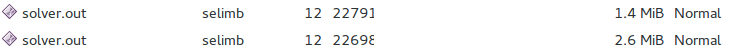
\includegraphics[width=0.8\textwidth]{./figs/memusage.png}}
    \caption{Memory usage (shown in second to last column) of Gauss (top) and Jacobi (bottom).
        The arrays containing times and residuals have not been allocated.
        The memory required by Gauss is roughly half of Jacobi's.}
    \label{fig:memusage}
\end{figure}



\newpage
\section{Question 6}
\begin{quote}
    \textit{Demonstrate that the order of accuracy of the scheme on a plot where the $y$-axis is the
log of the error and the $x$-axis is $\Delta x$, where both $\Delta x = \Delta y$.}
\end{quote}
\subsection{Analytical Solution}
In order to get values for the error, the analytical solution must be determined.

The solution to the Laplace equation on a unit square with Dirichlet boundary condtion $u = 0$ everywhere
except $y = 1$, where the condition is $f(x)$ for $0 \le x \le 1$ is given by the following:
\begin{align}
    \label{eq:uexg}
    U(x,y) &= \sum_{n=1}^\infty c_n \sinh(n \pi y) \sin(n \pi x)\\
    \label{eq:cg}
    \text{where} c_n &= 2 \int_0^1 f(x)\frac{\sin(n \pi x)}{\sinh(n\pi)} \text{d}x
\end{align}
\Cref{eq:cg} can be evaluated analytically with $f(x) = 1$:
\newcommand{\csol}[1]{- \frac{2\cos(#1 \pi) - 2}{#1 \pi \sinh(#1 \pi)}}

\begin{equation}
    \label{eq:c}
    c_n = \csol{n}
\end{equation}
which vanishes for even-numbered $n$!

Finally, substituting the above $c_n$ into~\Cref{eq:uexg} yields the exact field $U$ for this problem:
\begin{equation}
    \label{eq:uex}
    U(x,y) = \sum_{n=0}^\infty \csol{k}\sinh(k \pi y) \sin(k \pi x)
\end{equation}
where $k = 2n + 1$

\subsubsection{Implementation on a computer}
The series in \Cref{eq:uex} cannot be evaluated in its entirety on a computer for two reasons:
\begin{enumerate}[noitemsep]
    \item We cannot go to $\infty$.
    \item $\sinh(n\pi)$ eventually grows beyond the machine's largest representable number.
\end{enumerate}
The second item is the most problematic, since even going further than $n=223$ is made impossible when
using double precision.
Switching to 128 bit floating point numbers (quadruple-precision) allows us to reach
numbers as high as $1.2\text{e}+4392$ and as low as $1.1\text{e}-19$. Consequently, it becomes possible to sum
up to $n = 3611$, at which point \texttt{nan}s start showing up again.

Now, this lack of accuracy in the numerical analytical solution $U_{NA}$ is still a problem. However,
the results are smooth over the whole problem domain with the exception of the boundary $y = 1$. This is
illustrated in~\Cref{fig:topanal}. Since we know our finite difference approximate solution satisfies
the boundary conditions exactly, we can either ignore the top boundary in our error calculation or
manually enforce $U_{NA}(x,1) = 1$ after the fact.

\begin{figure}
    \centering
    \includegraphics[width=0.7\textwidth]{./figs/topanal}
    \caption{Approximation of the analytical solution $U_{NA}$ at $y = 1$ by evaluating
        the first 3611 terms of the infinite series.}\label{fig:topanal}
\end{figure}

\subsection{Error calculation}
\newcommand{\norm}[1]{\big|\big|#1\big|\big|}
The error is calculated as follows:
$$
e = \frac{\norm{U - U_{NA}}_1}{\norm{U_{NA}}_1}
$$
The 1-norm is used because it tends to be more resistant to outliers in the data, which is certainly the case
here. This can be observed in~\Cref{fig:errplot}. Indeed, errors are largest at the top left and right corners
but relatively low otherwise. Using a 2-norm would give significantly more weight to the larger error in those
regions.
\begin{figure}[H]
    \centering
    \includegraphics[width=0.8\textwidth]{./figs/errplot}
    \caption{Contour of $U - U_{NA}$ on a log scale. Highest errors are localized in the top corners.}
    \label{fig:errplot}
\end{figure}

\subsection{Comparison with approximation}
In order to truly obtain converged solutions and actually observe the effect of grid refinement, the tolerance
needed to be set to 10$^{-15}$.

\Cref{fig:orderaccuracy} shows the improvement in accuracy with grid refinement. The first thing we notice
is how values for Jacobi, Gauss and SOR are identical for each grid. This is the only thing that makes sense:
the linear solving technique should not affect the order of accuracy since it does not affect the equations
to solve whatsoever.
In other words, the coefficient matrix $A$ and right-hand side vector $b$ are not a result of the chosen
linear solver.

The order of accuracy is dictated by the spatial discretization scheme used, which remained the same
throughout all experiments for this report. Now, it was derived in Question 1 that the finite difference
scheme used is second-order accurate. Thus, the truncation error varies as $O(\Delta x^2, \Delta y^2)$.
Thus, since the grid is refined uniformly both in the $x$ and $y$, we can simply say
that the error decreases as $O(\Delta x^2)$.

Thus, it is expected that the slope on a log plot of the error versus the number of grid points be close to
2. The actual slope is shown on the graph and is relatively close to 2 -- it's closer to 2 than it is to 1.
The fact that our scheme is second-order is confirmed.
\begin{figure}[H]
    \centering
    \includegraphics[width=0.7\textwidth]{./figs/orderaccuracy}
    \caption{Error vs. number of grid points on a log scale with a straight line fit.}\label{fig:orderaccuracy}
\end{figure}



\newpage
\section{Question 7}
\begin{quote}
    \textit{Effect of the relaxation parameter on the SOR. Try several different values and discuss
    your findings. Show plots of the convergence of the residual for various relaxation
    parameters. Is there an optimum relaxation parameter? Is the optimum the same for
    all grid sizes.}
\end{quote}
Refer to~\Cref{fig:q7} for plots of the convergence of the residual for various values of $\omega$
on all grid sizes.
\begin{figure}
    \centering
    \includegraphics[width=1.0\textwidth]{./figs/q7.pdf}
    \caption{Effect of relaxation parameter on convergence rate for $N = 100, 200, 400$ going from top to bottom.}
    \label{fig:q7}
\end{figure}

In all previous questions, SOR essentially acted as an over-relaxed Gauss scheme. This leads to quicker
convergence, since the ``correction'' at each point is attributed a greater weight.
In other words, values are allowed to vary faster. Of course, over-relaxation is not the
best choice for every problem. In fact, under-relaxation is often necessary when dealing with stiff
problems. A more detailed discussion on relaxation is, however, beyond the scope of this assignment and course.

The higher the relaxation parameter, the better. This applies to all grid sizes. However, it was found that 2
is an upper bound for stability. In other words, setting $\omega \ge 2$ leads to
large spurious oscillations in the residual and a complete lack of convergence.

\newpage
\appendix
\section{Appendix}
\subsection{Optimization and Performance}
\Cref{tab:performance} illustrates the effects of optimization level on performance for the Jacobi and Gauss schemes.
\newcommand{\mct}[1]{\multicolumn{2}{c}{#1}}
\newcommand{\pht}{\phantom{a}}
\newcommand{\mrt}[1]{\multirow{4}{*}{#1}}
\begin{table}[H]
\caption{Performance comparison of Gauss and Jacobi using different
optimization levels. All runs converged with a tolerance of
$10^{-6}$.}
\label{tab:performance}
\centering
\begin{tabular}{@{}r cc c cc c cc @{}}
    \toprule
    & \mct{Iterations} & \pht & \mct{Time per Iteration} & \pht & \mct{Total Time}\\
    &         &        & \pht & \mct{($10^{-5}$ s)}        & \pht & \mct{(s)}       \\
    \cmidrule{2-3} \cmidrule{5-6} \cmidrule {8-9}
     & Jacobi & Gauss && Jacobi & Gauss && Jacobi & Gauss\\
    \midrule

$N = 100$\\
     g & \mrt{10726} & \mrt{6020} && 24 & 23 &&  2.53 &  1.38 \\
    O1 &  &  && 8 & 9 &&  0.91 &  0.53 \\
    O2 &  &  && 6 & 7 &&  0.68 &  0.41 \\
    O3 &  &  && 4 & 6 &&  0.38 &  0.39 \\
$N = 200$\\
     g & \mrt{31851} & \mrt{18684} && 93 & 93 &&  29.7 &  17.3 \\
    O1 &  &  && 34 & 35 &&  10.7 &   6.6 \\
    O2 &  &  && 25 & 27 &&   8.1 &   5.1 \\
    O3 &  &  && 14 & 26 &&   4.5 &   4.9 \\
$N = 400$\\
     g & \mrt{83206} & \mrt{52634} && 375 & 371 &&   312 &   195 \\
    O1 &  &  && 135 & 142 &&   112 &    75 \\
    O2 &  &  && 102 & 109 &&    85 &    58 \\
    O3 &  &  && 57 & 107 &&    47 &    56 \\

    \bottomrule
\end{tabular}
\end{table}

\subsection{Linear Solver Code}
The meat of the code is shown below. The call to the \texttt{update} subroutine is inside a \texttt{while} loop.

The only difference between Jacobi and Gauss-Siedel is the allocation
of a \texttt{uold} array and its usage in calculating \texttt{s}, the multiplier of $a_{ij}$.

In fact, Jacobi probably could've been made faster if the allocation wasn't done at every iteration, which is currently
the case.

\lstset{language=[90]Fortran,
  basicstyle=\footnotesize\ttfamily,
  lineskip=-2pt,
  frame=single,
  keywordstyle=\color{blue},
  commentstyle=\color{PineGreen},
  numbers=left,
  morecomment=[l]{!\ }% Comment only with space after !
}
The listing below shows the meat of the code.
\texttt{implicit none} is used,
which means all undeclared variables that appear in the listing are globals.
These globals are all constants.
\begin{lstlisting}[caption={Relevant part of the linear solver.
\texttt{solverID} is a global integer variable that has the mapping:
1=Jacobi, 2=Gauss, 3=SOR},
label=lst:fortran]
subroutine update(u, maxerr)
    real(sp), dimension(:), intent(inout) :: u
    real(sp), intent(out) :: maxerr
    real(sp), allocatable, dimension(:) :: uold
    real(sp) :: s, corr, err
    integer, dimension(4) :: stencil
    integer :: i, j, row
    maxerr = 0
    if (solverID .eq. 1) then
        allocate(uold(size(u)))
        uold = u
    end if
    do i = 1, nx
        do j = 1, nx
            if (is_bc(i,j)) then
                cycle
            end if
            row = get_row(i, j)
            ! Calculate correction
            stencil = (/ row-nx, row-1, row+1, row+nx /)
            if (solverID .eq. 1) then
                s = sum(uold(stencil))
            else
                s = sum(u(stencil))
            end if
            corr = (BI - AIJ*s)/AII
            if (solverID .eq. 3) then
                corr = (1.0 - relax)*u(row) + relax*corr
            end if
            ! Calculate error
            err = abs(corr - u(row))
            maxerr = max(maxerr, err)
            ! Assign correction
            u(row) = corr
        end do
    end do
end subroutine
\end{lstlisting}

\subsection{Cache Calculations}
These are rough calculations and based on my limited computer science knowledge.

My personal computer has an L3 cache size of 6MB. For a $N = 400$ problem, a $u$ array is of length $400^2$.
Using single precision -- a single precision floating point number takes up 4 bytes -- this means $u$ takes up
0.64MB.  Thus, storing an additional \texttt{uold} array should not be a problem.

I also tried bumping $N$ up to 1000 -- which brings the size of $u$ to 4MB -- and Jacobi
was \textit{still} faster than Gauss at O3, although the time per iteration ratio (Gauss/Jacobi) increased
from 0.53 (for $N = 400$) to 0.73, meaning the optimization was not as significant. However, Jacobi wasn't any
slower than Gauss at O2 or O1 either.

Thus, all we can conclude is that my understanding of cache is not great and that increasing $N$ will
apparently not make Jacobi slower.
\end{document}
